\section{Continual Learning in Agents}
\begin{frame}{}
  \LARGE Continual Learning in Agents
\end{frame}

\begin{frame}{Continual Learning in Agents}
  \begin{figure}
    \centering
    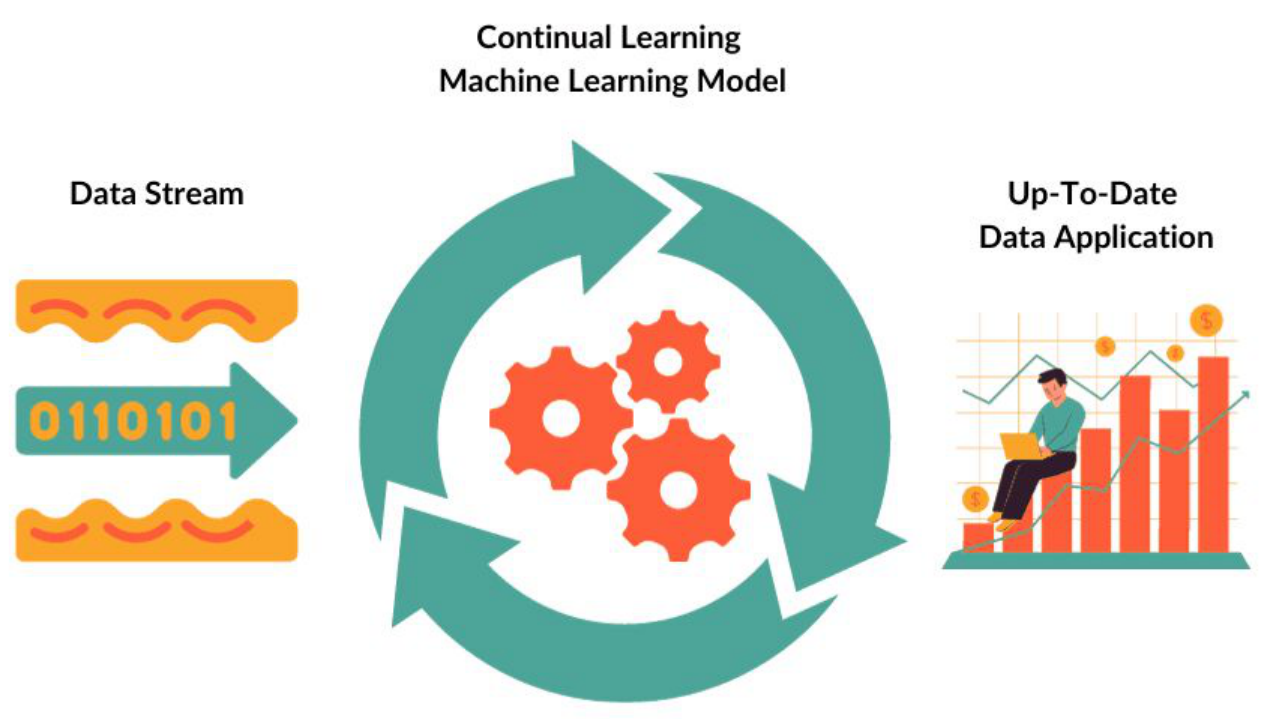
\includegraphics[width=0.98\textwidth,height=0.76\textheight,keepaspectratio]{images/multimodal-nlp-agentic-ai/agentic_continual_learning_cycle.png}
    \caption*{\scriptsize Source: N.~Van Otten, ``Continual Learning Made Simple, How To Get Started \& Top 4
    Models'', Spot Intelligence, 2023.}
  \end{figure}
\end{frame}

\begin{frame}{Why Continual Learning?}
  \begin{itemize}
    \item[\textcolor{red}{$\triangleright$}] \textbf{Agentic AI should evolve with time:}
    \begin{itemize}
      \item[\textcolor{red}{$\bullet$}] Learn from feedback
      \item[\textcolor{red}{$\bullet$}] Adapt to new tasks
      \item[\textcolor{red}{$\bullet$}] Retain useful knowledge
    \end{itemize}

    \vspace{1em}
    \item[\textcolor{red}{$\triangleright$}] \textbf{Real-world scenarios:}
    \begin{itemize}
      \item[\textcolor{red}{$\bullet$}] \textbf{Personalization:} the same assistant serving one user for a year.
      \item[\textcolor{red}{$\bullet$}] \textbf{Environment drift:} tools, APIs, and documents change under the agent.
      \item[\textcolor{red}{$\bullet$}] \textbf{Avoiding forgetting:} new skills must not erase old ones.
    \end{itemize}
  \end{itemize}
\end{frame}

\begin{frame}{Challenges in Continual Learning}
  \begin{itemize}
    \item[\textcolor{red}{$\triangleright$}] \textbf{Catastrophic forgetting:} Agents may lose previously acquired knowledge when learning new tasks.
    \item[\textcolor{red}{$\triangleright$}] \textbf{Stability-plasticity dilemma:} Balancing the ability to learn new information (plasticity) with retaining old knowledge (stability).
    \item[\textcolor{red}{$\triangleright$}] \textbf{Modality drift:} Changes in the types or distributions of input modalities over time.
    \item[\textcolor{red}{$\triangleright$}] \textbf{Scaling memory:} Managing both semantic (general knowledge) and episodic (specific experiences) memory as agents interact with the world.
  \end{itemize}

  \textbf{Solutions:}
  \begin{itemize}
      \item \textbf{Experience replay:} interleave a buffer of past examples with the new ones, so old
        tasks keep contributing gradient.
      \item \textbf{Progressive networks:} freeze the trained columns and add a fresh one per task, with
        lateral connections, so nothing is overwritten.
      \item \textbf{Elastic weight consolidation (EWC):} penalise moving the weights that mattered most
        for earlier tasks.
  \end{itemize}
\end{frame}

\begin{frame}{Catastrophic forgetting}
  \begin{figure}
    \centering
    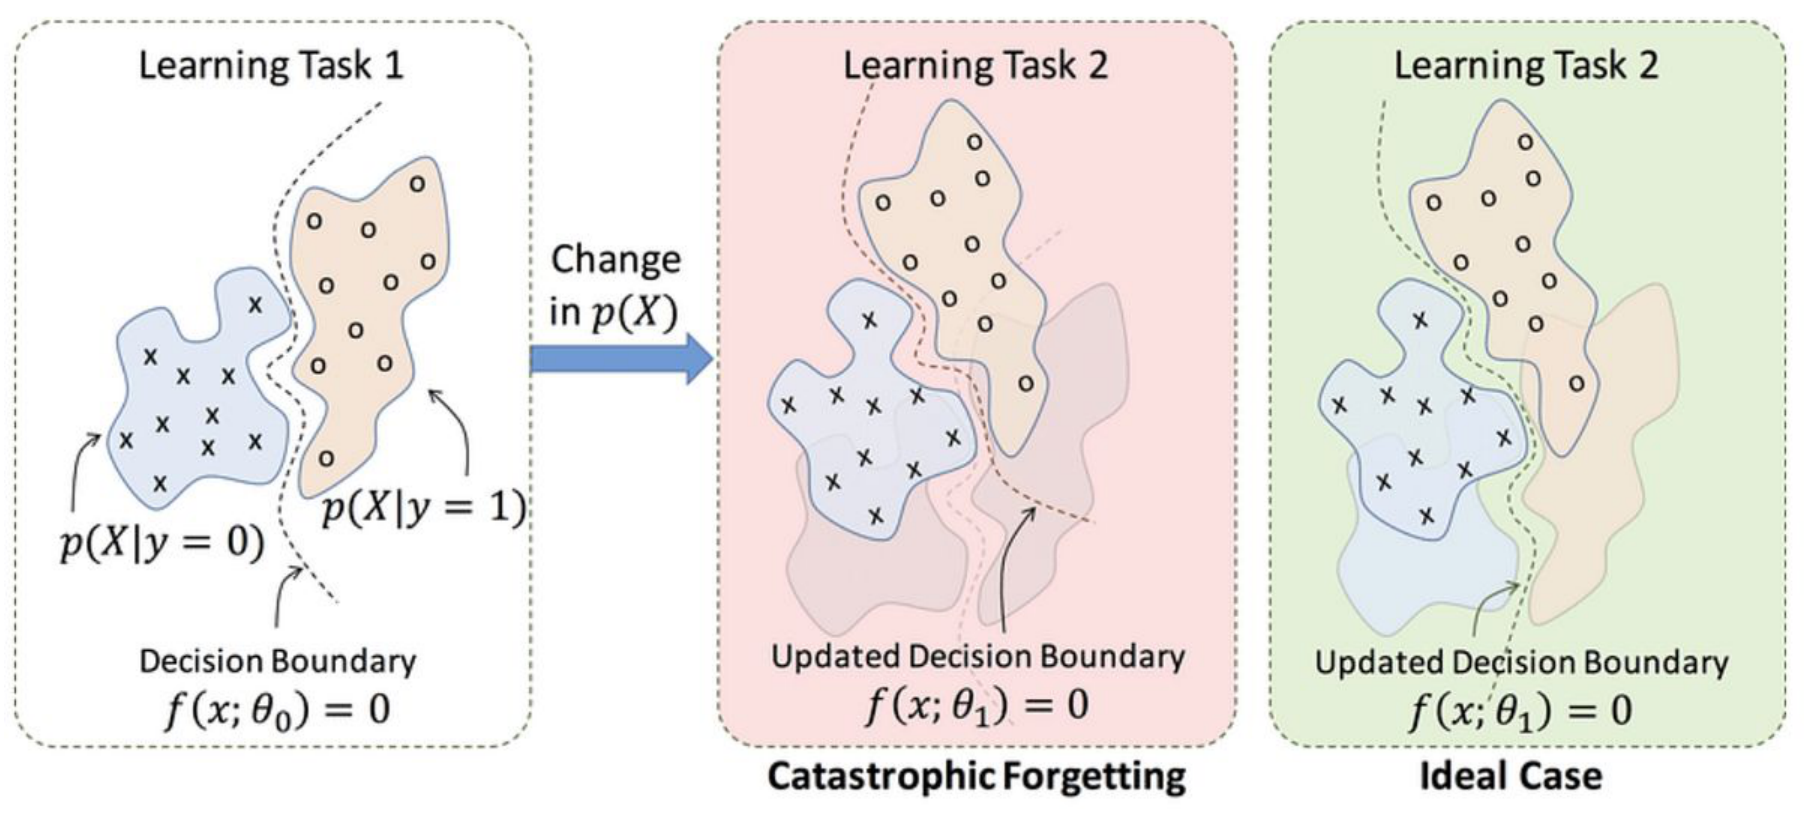
\includegraphics[width=0.98\textwidth,height=0.76\textheight,keepaspectratio]{images/multimodal-nlp-agentic-ai/agentic_catastrophic_forgetting.png}
    \caption*{\scriptsize Source: Kolouri, Ketz, Zou, Krichmar \& Pilly, ``Attention-Based Selective
    Plasticity'', \href{https://arxiv.org/abs/1903.06070}{arXiv:1903.06070}, Figure~1.}
  \end{figure}
\end{frame}

\begin{frame}{Catastrophic forgetting}
  \begin{figure}
    \centering
    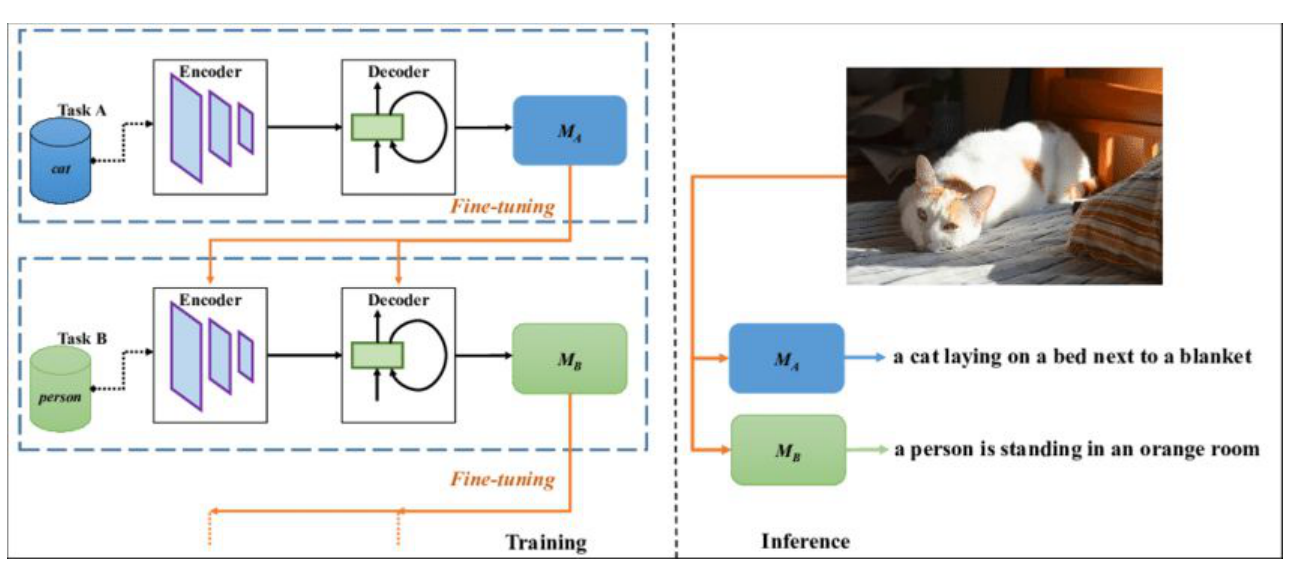
\includegraphics[width=0.98\textwidth,height=0.76\textheight,keepaspectratio]{images/multimodal-nlp-agentic-ai/agentic_continual_learning_captioning.png}
    \caption*{\scriptsize After fine-tuning on task B, the same cat photograph is captioned ``a person is
    standing in an orange room''. Source: Nguyen et al., ``ContCap: A scalable framework for continual image
    captioning'', \href{https://arxiv.org/abs/1909.08745}{arXiv:1909.08745}.}
  \end{figure}
\end{frame}

\begin{frame}{Stability-plasticity dilemma}
  \begin{figure}
    \centering
    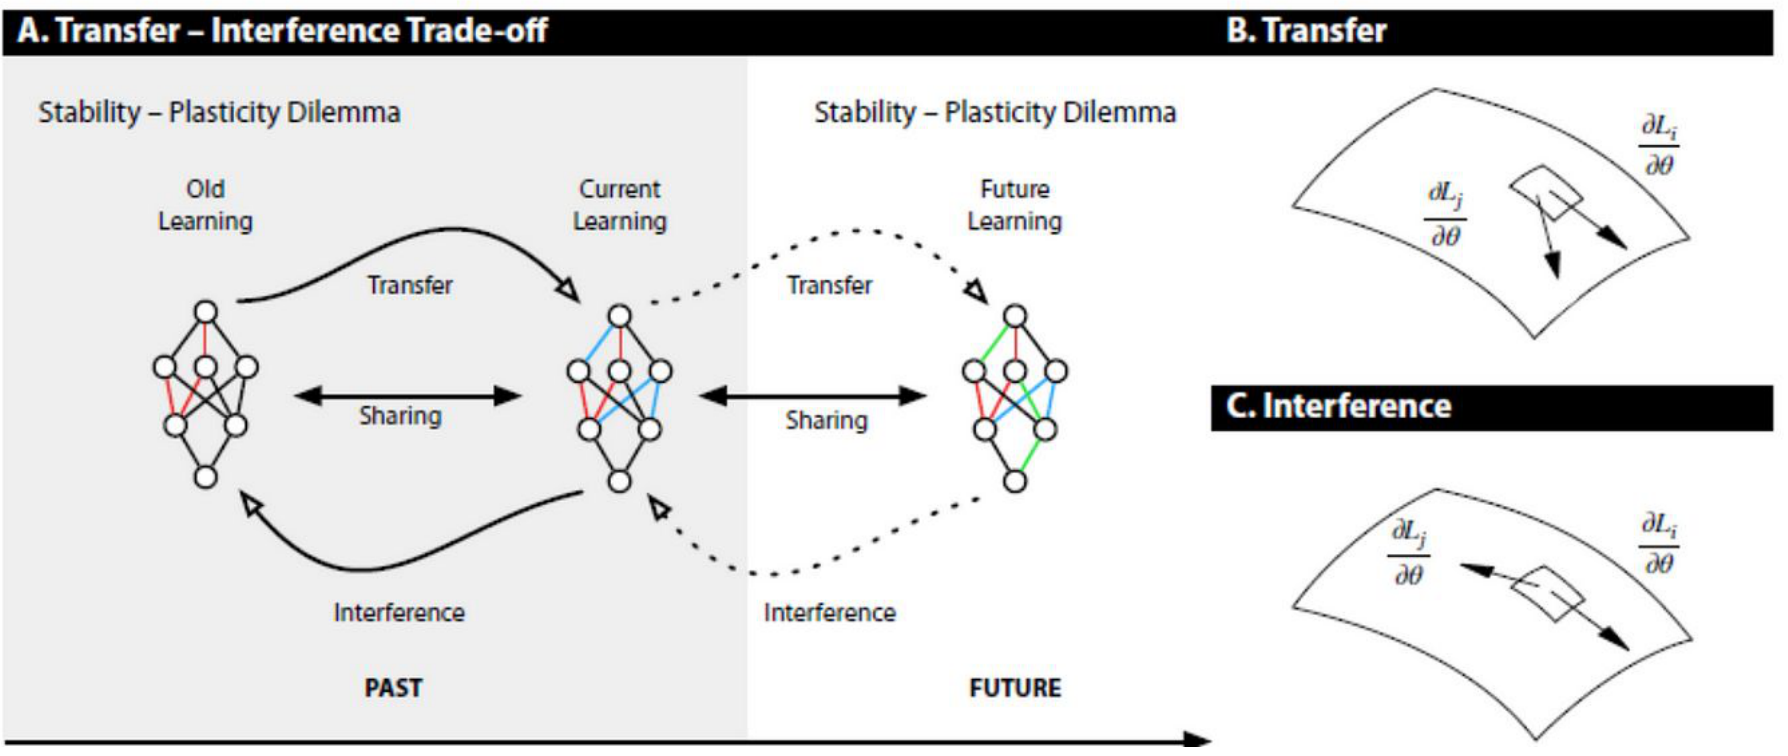
\includegraphics[width=0.98\textwidth,height=0.76\textheight,keepaspectratio]{images/multimodal-nlp-agentic-ai/agentic_stability_plasticity_dilemma.png}
    \caption*{\scriptsize Gradients that point the same way across tasks give transfer; gradients that
    oppose give interference. Source: Riemer et al., ``Learning to Learn without Forgetting by Maximizing
    Transfer and Minimizing Interference'', ICLR 2019,
    \href{https://arxiv.org/abs/1810.11910}{arXiv:1810.11910}, Figure~1.}
  \end{figure}
\end{frame}

\begin{frame}{Scaling memory}
  \begin{figure}
    \centering
    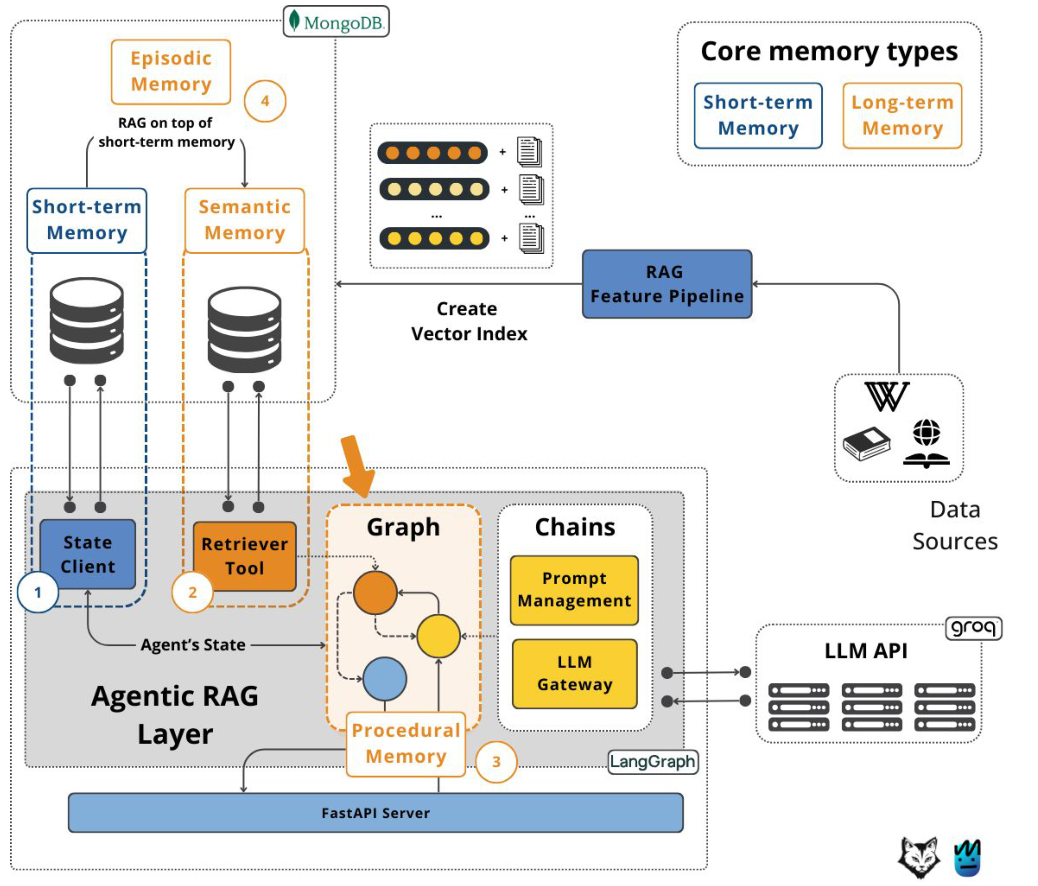
\includegraphics[width=0.8\textwidth,height=0.72\textheight,keepaspectratio]{images/multimodal-nlp-agentic-ai/agentic_rag_memory_architecture.png}
    \caption*{\scriptsize Source: P.~Iusztin, ``Memory: The Secret Sauce of AI Agents'', Decoding AI, 2025.}
  \end{figure}
\end{frame}
